
%(BEGIN_QUESTION)
% Copyright 2015, Tony R. Kuphaldt, released under the Creative Commons Attribution License (v 1.0)
% This means you may do almost anything with this work of mine, so long as you give me proper credit

\noindent

\vskip 5pt



\vskip 5pt
\begin{center}
\textbf{Kommunikkasjon -- Nivå 1 }
\vskip 5pt 
\textbf{Arbidsoppdrag på Stasjon 2}
\vskip 5pt 
\textbf{Oppkobling med Profinet til RIO Sjekk av komunkasjonsnett i klasserommet}
\end{center}
\vskip 5pt 
\vskip 5pt 
\textbf{Introduksjon}

Målet med oppgaven er å lære hvordan vi kobler opp en PLS til en profinet RIO.

$$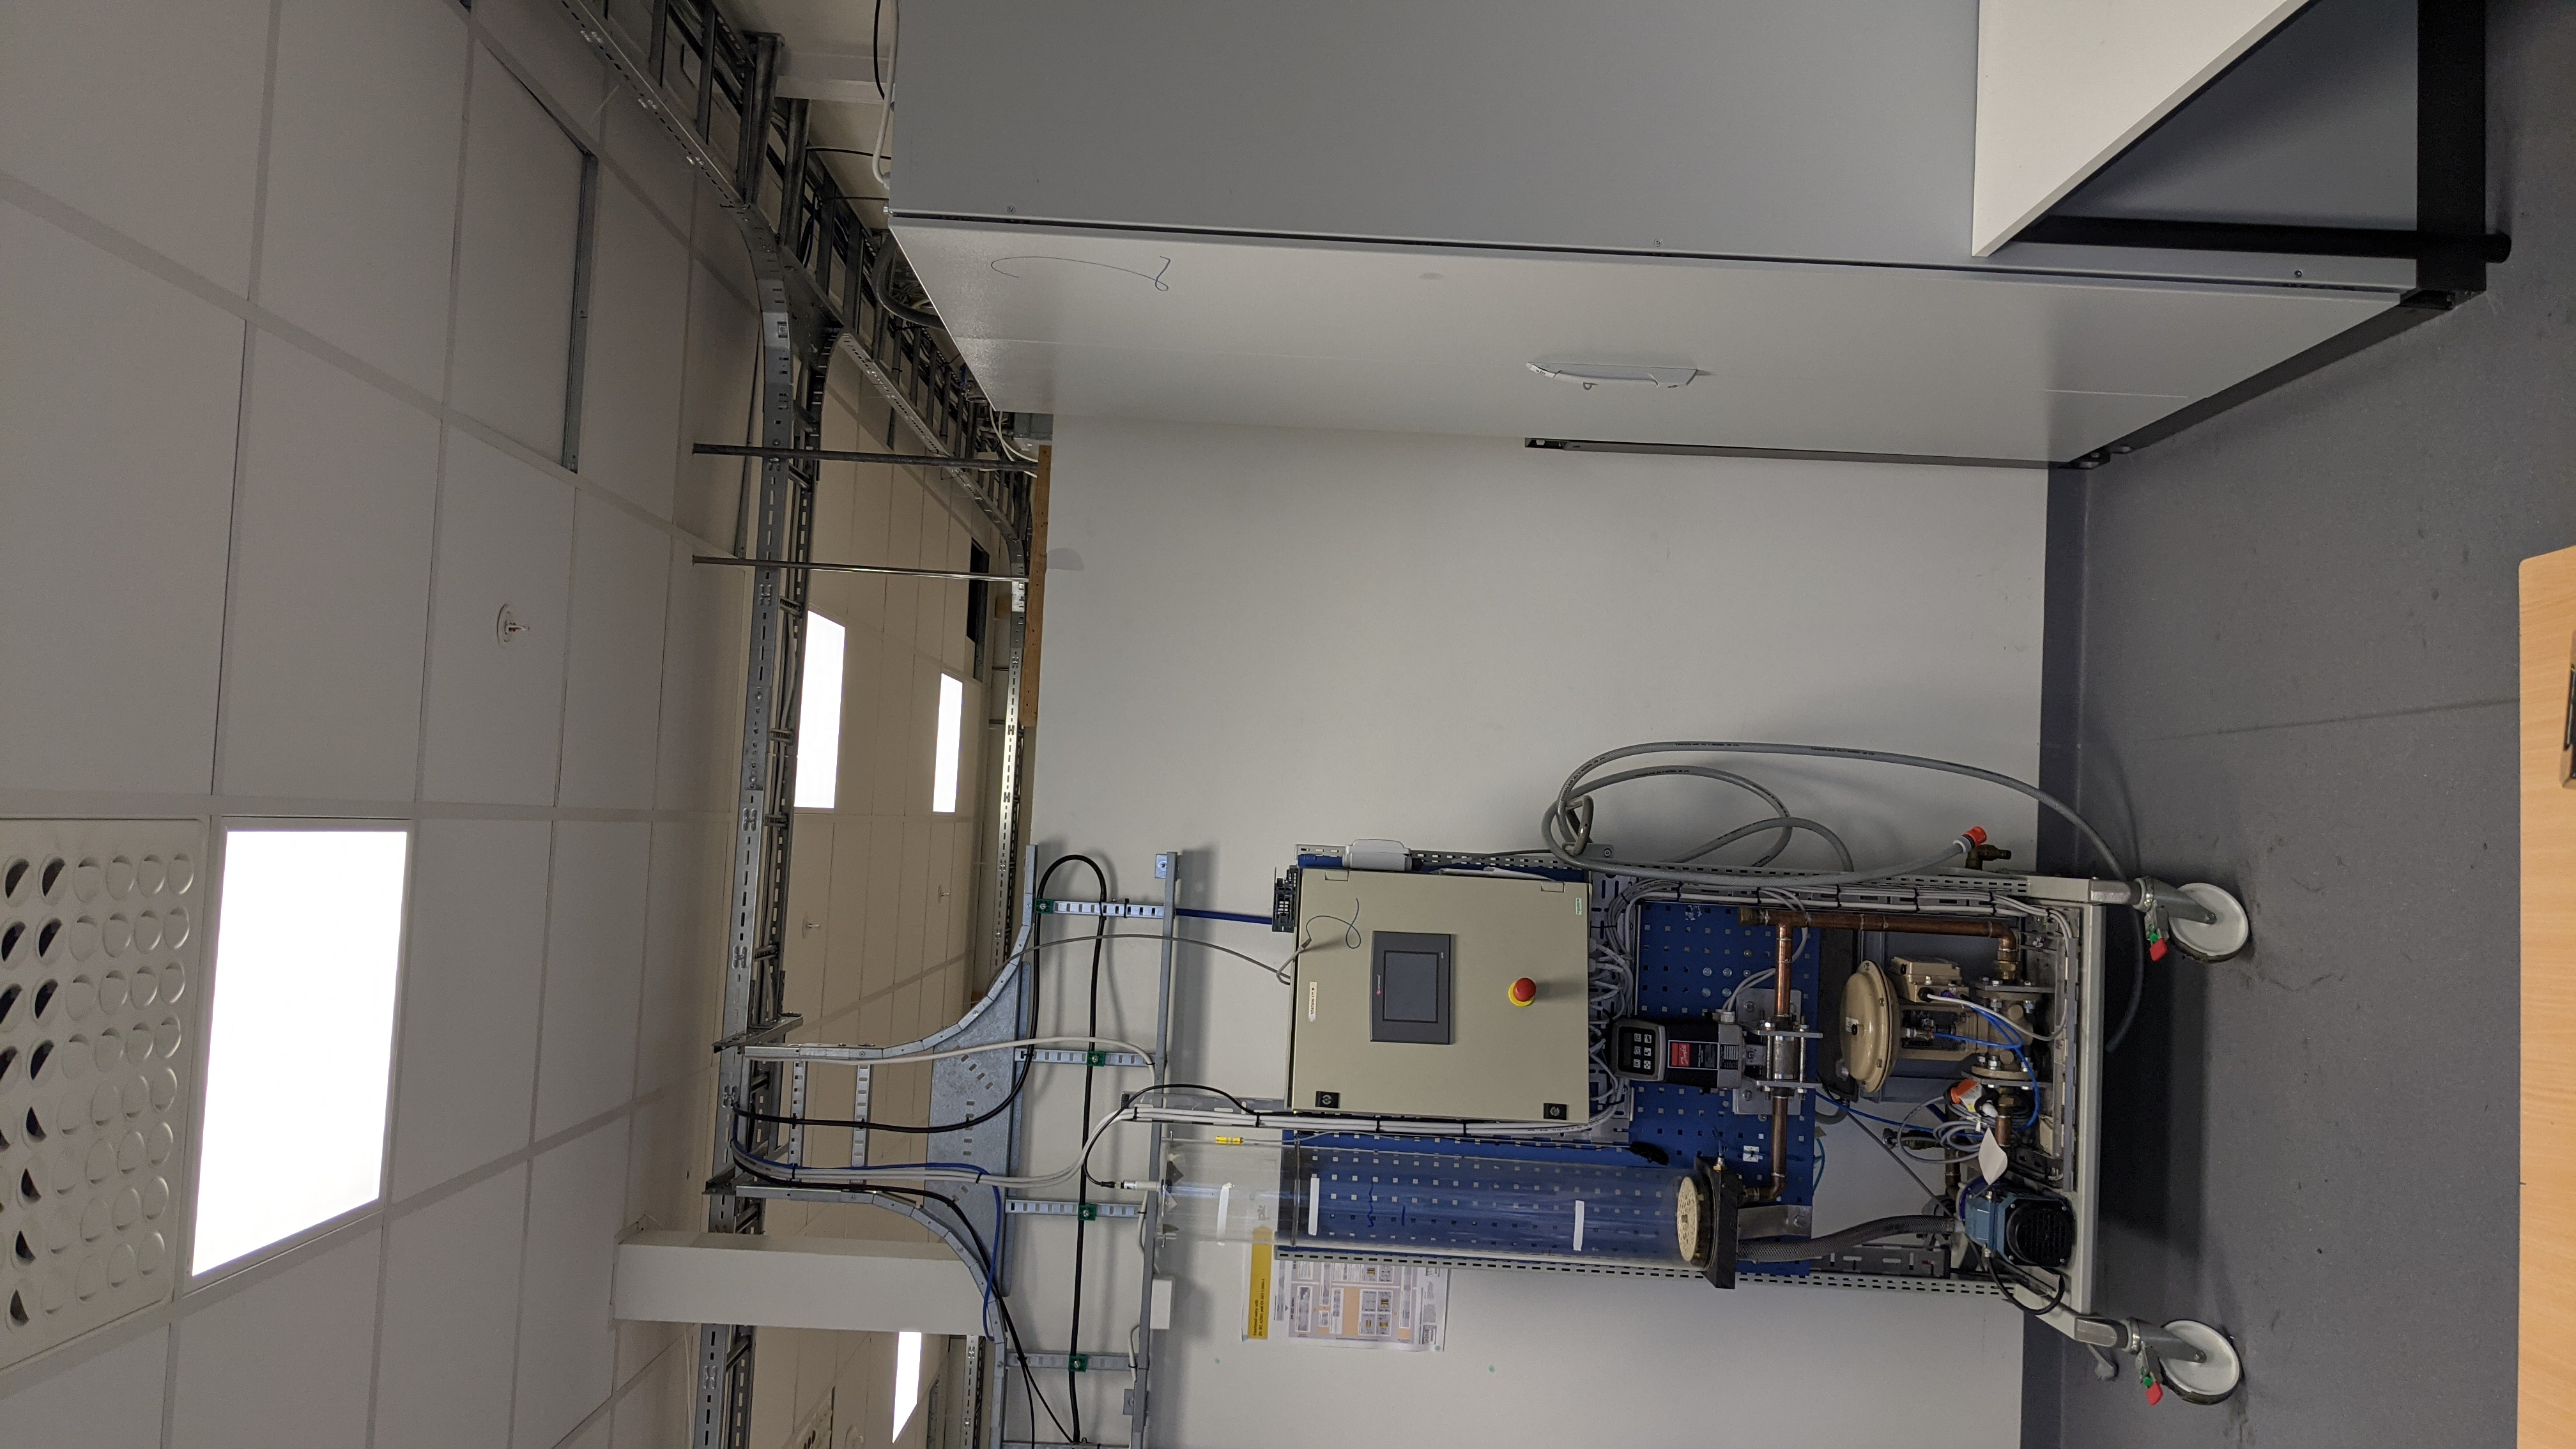
\includegraphics[width=10.5cm,angle=-90]{stasjon02x01.jpg}$$


\textbf{Arbidsoppdrag -- teorioppgaver}

\begin{enumerate}
	\item Sett deg inn i manualen til aktuell DP-celle
\end{enumerate}
\textbf{Arbidsoppdrag -- planlegging}

Utstyr:
\begin{itemize}[noitemsep]
	\item Egen pc med codesys installert 
\end{itemize}

\textbf{Arbidsoppdrag -- gjennomføring}
Profinet 

 

Installer CODESYS 3.5 V17 

Installer WinPcap version is 4.1.3  (https://www.winpcap.org/install/default.htm ), denne finner du også i fagbiblioteket. 


$$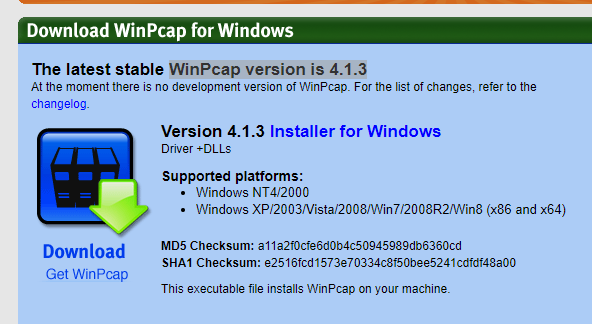
\includegraphics[width=13cm]{i04834x1.png}$$\\
Restart PC \\
Start CODESYS \\
Installer GSD fil for Siemens IM153-4 \\
$$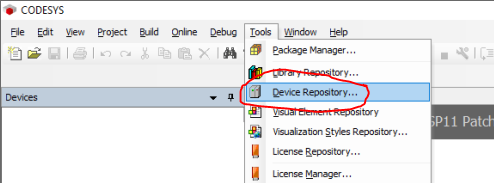
\includegraphics[width=13cm]{i04834x2.png}$$\\
$$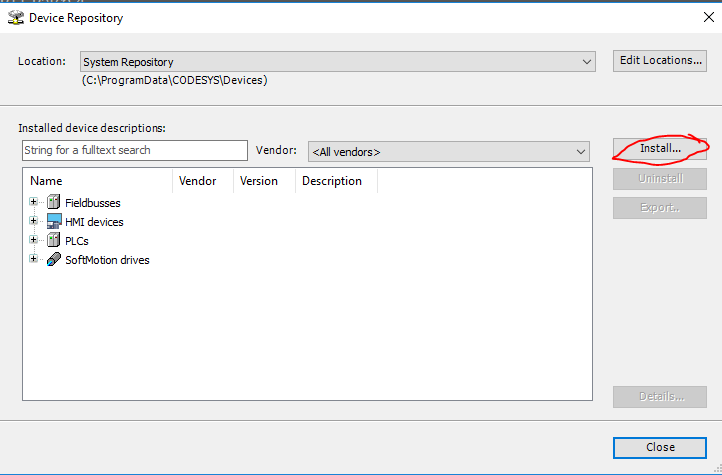
\includegraphics[width=13cm]{i04834x3.png}$$\\
Velg denne lokasjonen i fagbiblioteket \\
$$
\includegraphics[width=13cm]{i04834x4.png}$$\\
$$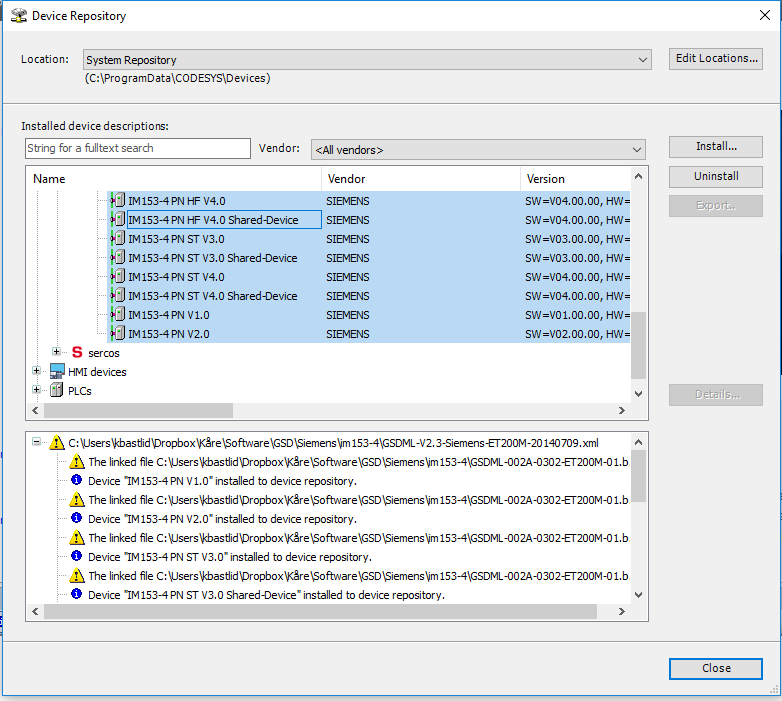
\includegraphics[width=13cm]{i04834x5.png}$$\\
Lukk vinduet etter installasjonen er fullført \\
Lag et nytt prosjekt MCI2 Profinet  \\
Legg til Profinet \\
$$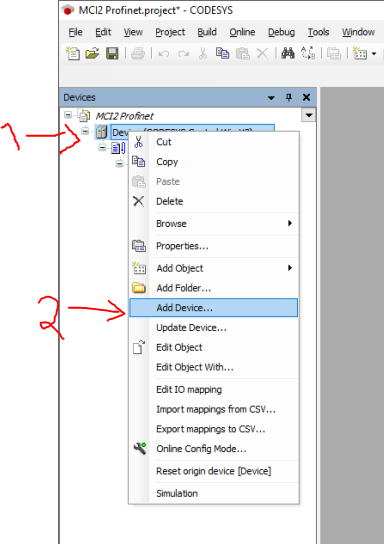
\includegraphics[width=13cm]{i04834x6.png}$$\\
$$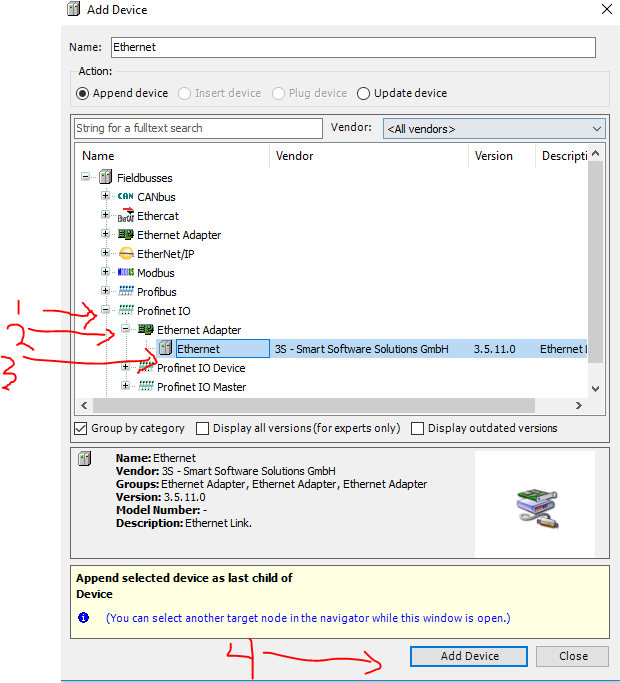
\includegraphics[width=13cm]{i04834x7.png}$$\\
$$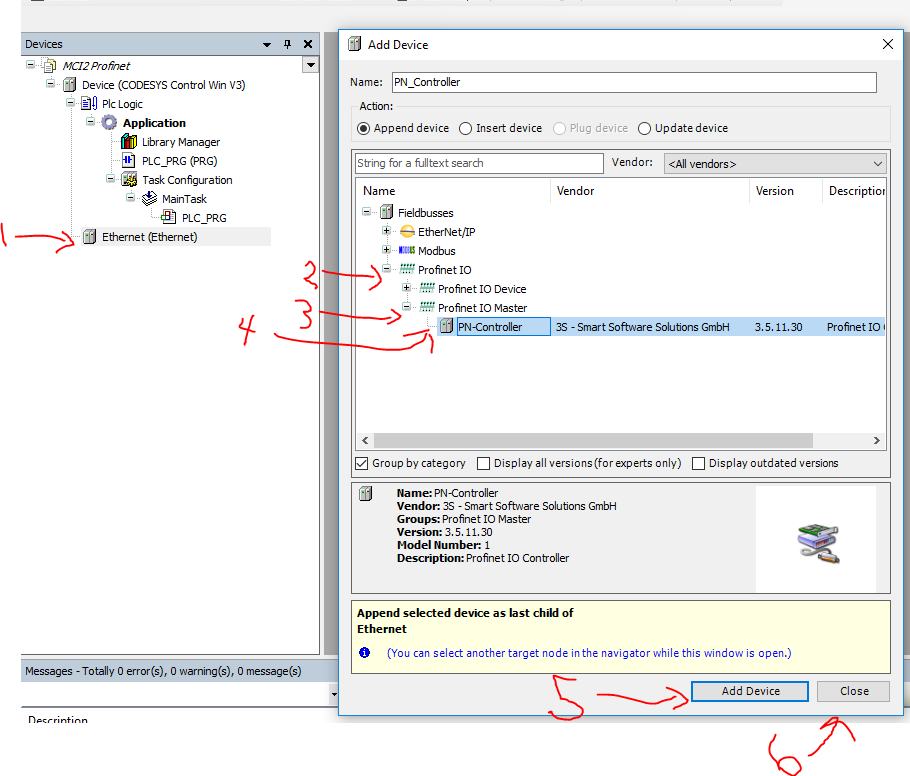
\includegraphics[width=13cm]{i04834x8.png}$$\\
Start PLC \\
$$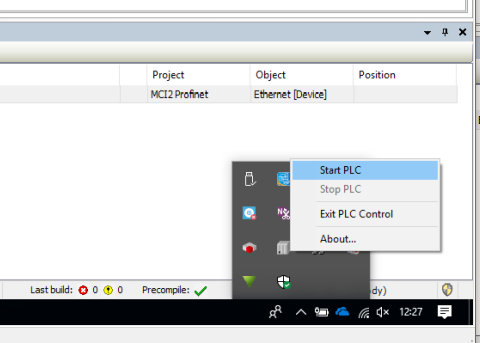
\includegraphics[width=13cm]{i04834x9.png}$$\\
$$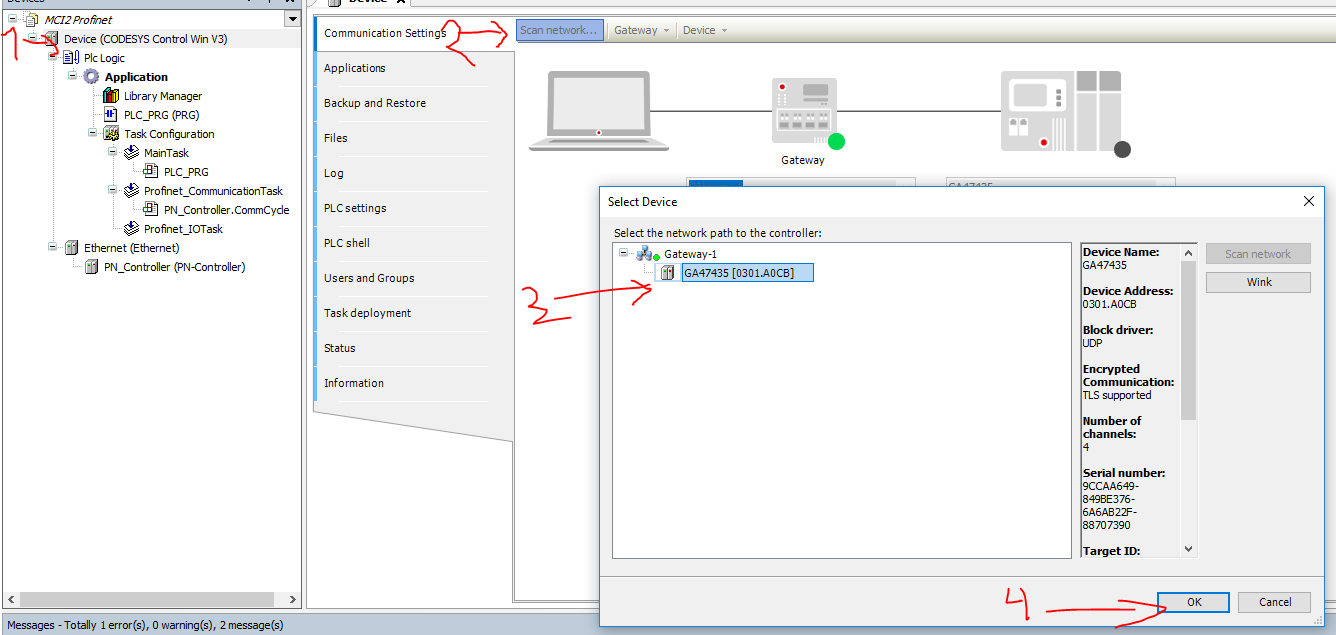
\includegraphics[width=13cm]{i04834x10.png}$$\\
$$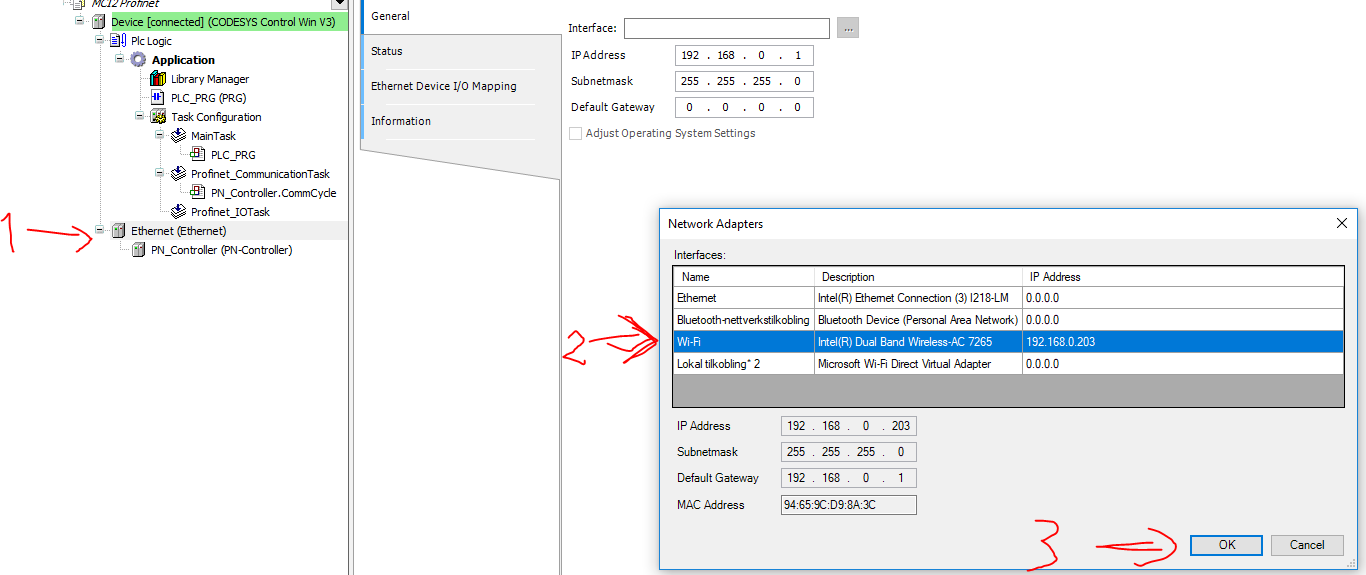
\includegraphics[width=13cm]{i04834x11.png}$$\\
Om du bruker kabel må du velge Ethernet i istedenfor.  \\
$$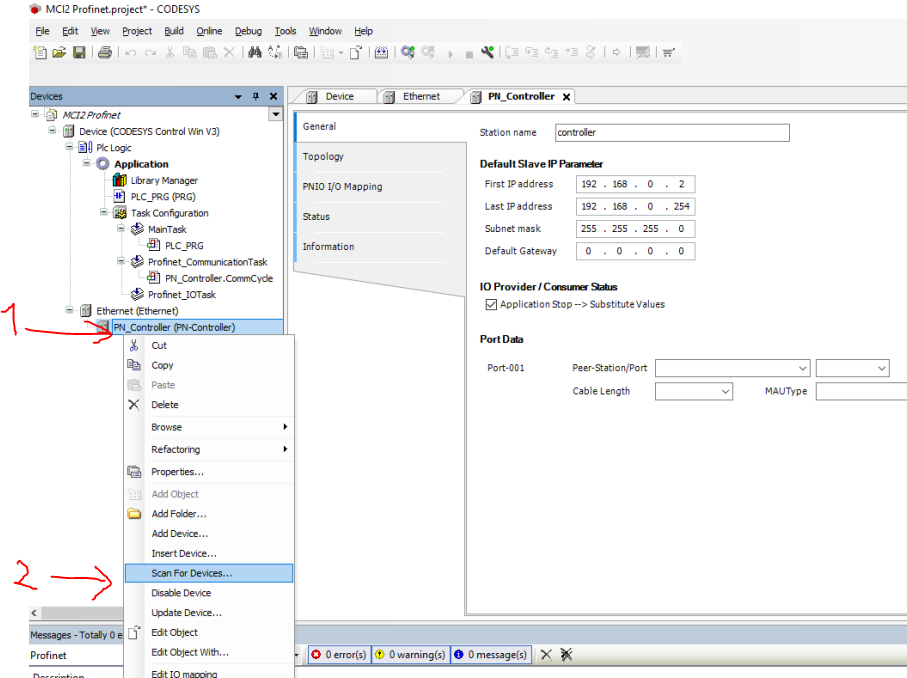
\includegraphics[width=13cm]{i04834x12.png}$$\\
$$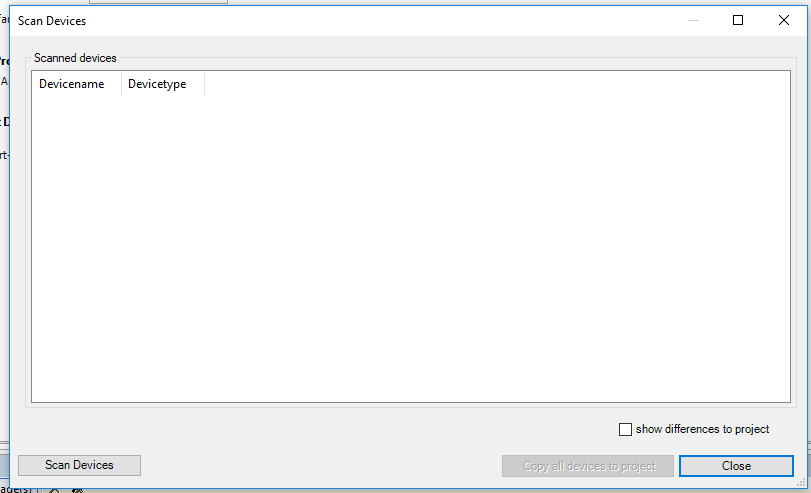
\includegraphics[width=13cm]{i04834x13.png}$$\\
$$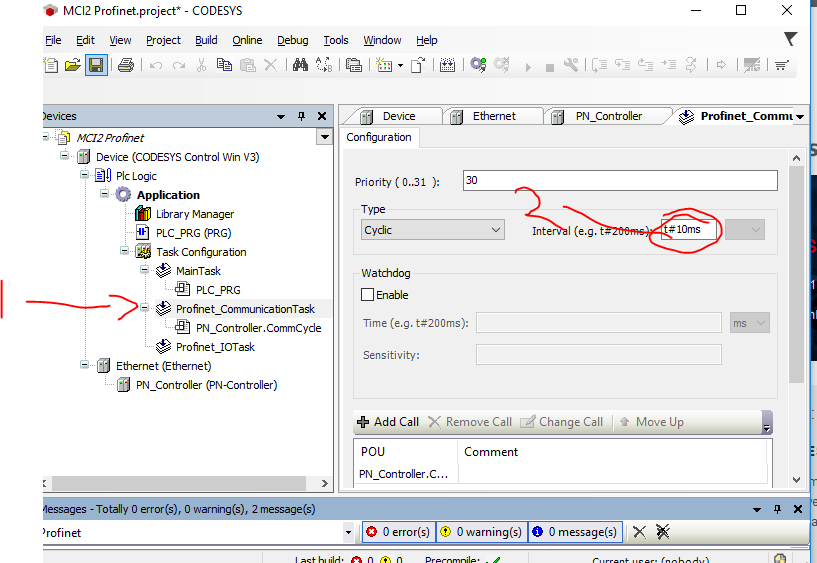
\includegraphics[width=13cm]{i04834x14.png}$$\\
Set tiden til 4ms, det er den høyeste tiden IM153-4 kjører. \\
Oppgaven \\
\\
						     \\

Få kontakt med PLS D22 og demonstrer for lærer at du kan sette utgangen og ta imot inngangssignaler.\\
\textbf{Arbidsoppdrag -- dokumentasjon}\\

\begin{enumerate}
	\item Beskriv hvordan du planla, gjennomførte og dokumentere jobben. Forklar eventuelle avvik dere måtte observere under oppdraget. 
\end{enumerate}










\underbar{file i04834}
%(END_QUESTION)





%(BEGIN_ANSWER)


%(END_ANSWER)





%(BEGIN_NOTES)


%INDEX% Arbeisdoppdrag, Kommunikkasjon, Nivå 1, Stasjon02, Oppkobling, Profinet

%(END_NOTES)


